I \gls{Design Pattern} sono un modello da applicare per la risoluzione di problemi ricorrenti. Essi possono essere organizzati in quattro categorie:
\begin{itemize}
	\item \textbf{Architetturali}: dividono il sistema in sottosistemi specificandone le responsabilità e dettando linee guida per organizzare le relazioni tra loro;
	\item \textbf{Creazionali}: forniscono un'astrazione del processo d'istanziazione degli oggetti. Aiutano a rendere il sistema indipendente dalle modalità d'istanziazione, composizione e rappresentazione degli oggetti utilizzati;
	\item \textbf{Strutturali}: si occupano della composizione di classi ed oggetti per formare Strutture complesse;
	\item \textbf{Comportamentali}: si occupano della gestione degli algoritmi e delle responsabilità di oggetti che collaborano tra loro.
\end{itemize}

\subsection{Pattern Architetturali}
\begin{itemize}
	\item Model-View-Controller(\gls{MVC})
	\begin{itemize}
		\item \textbf{Descrizione:} prevede la separazione in tre componenti:
		\begin{itemize}
			\item \textit{model}: fornisce i metodi per accedere ai dati utili all'applicazione;
			\item \textit{view}:  visualizza i dati contenuti nel model e si occupa delle interazione esterne;
			\item \textit{controller}: esegue funzionalità chiamate dalle view e modifica lo stato di model e/o view.
		\end{itemize}
		\item \textbf{Contesto d'utilizzo:} \gls{Front-End} \newline È stato adottato perché permette di organizzare modularmente gli strati software mantenendo una struttura che permette di lavorare agevolmente con il \gls{framework} \gls{Angular}.js. Per l'utilizzo di questo framework è stata applicata una variazione al pattern in modo da inserire anche le componenti per le direttive e i servizi richiesti.
		\begin{figure}[h]
			\centering
			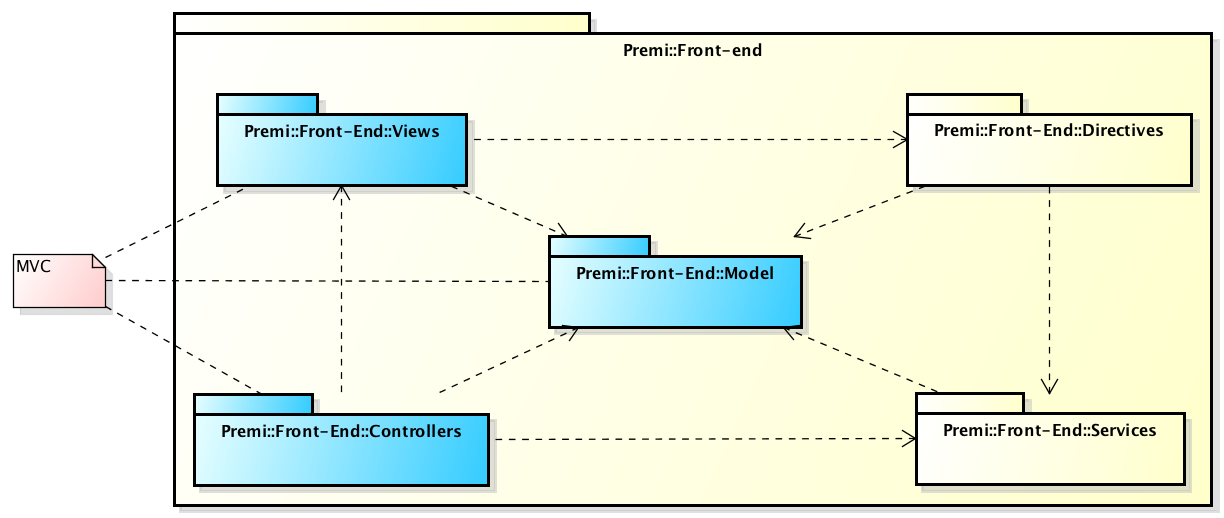
\includegraphics[width=\linewidth]{img/front-end_mvc}
			\caption[MVC Pattern - Premi::Front-End]{MVC Pattern - Premi::Front-End}
		\end{figure}
	\end{itemize}
\end{itemize}

\subsection{Pattern Strutturali}
\begin{itemize}
	\item Composite
	\begin{itemize}
		\item \textbf{Descrizione:} permette di comporre oggetti in strutture ad albero per rappresentare gerarchie in grado di trattare componenti foglia oppure composti allo stesso modo.
		\item \textbf{Contesto d'utilizzo:} Premi::Front-End::Model e Premi::Back-End::Model. È stato adottato nei model sia del \gls{Front-End} che del \gls{Back-End} per creare la struttura di un componente della slide. 
		\begin{figure}[h]
			\centering
			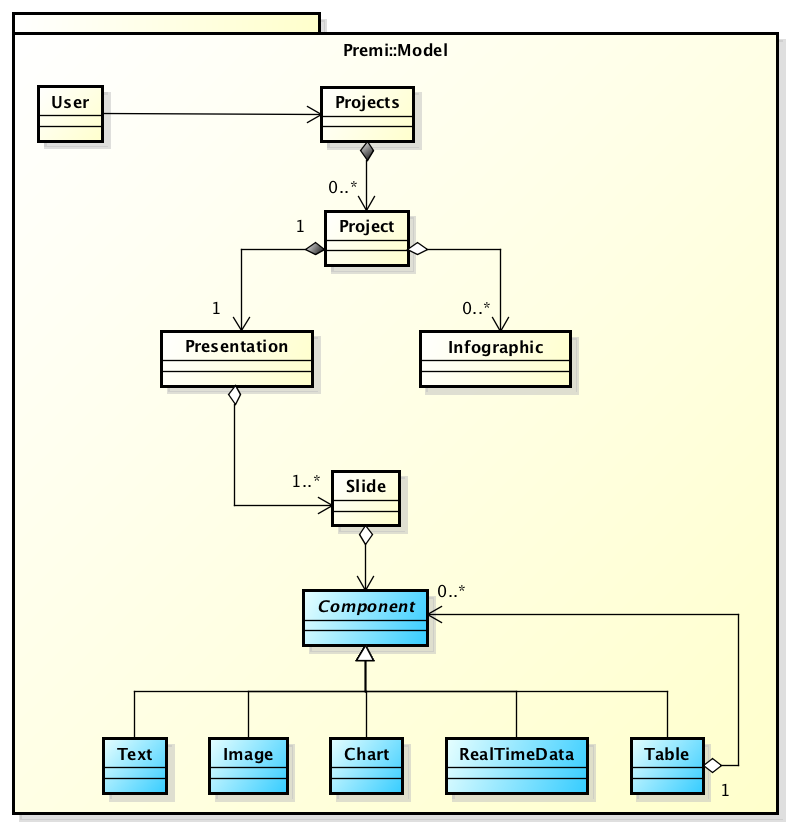
\includegraphics[width=0.5\linewidth]{img/front-end_model_composite}
			\caption[Composite Pattern - Premi::Front-End::Model]{Composite Pattern - Premi::Front-End::Model}
		\end{figure}
		\begin{figure}[h]
			\centering
			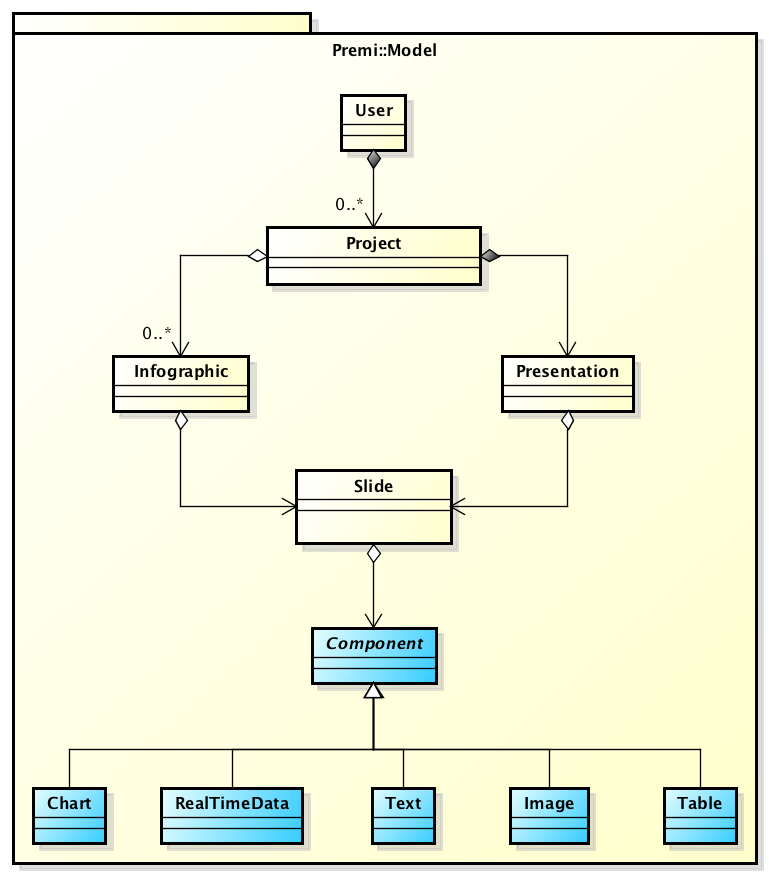
\includegraphics[width=0.5\linewidth]{img/back-end_logic-tier_premi_model_composite}
			\caption[Composite Pattern - Premi::Back-End]{Composite Pattern - Premi::Back-End}
		\end{figure}
	\end{itemize}

\end{itemize}

\subsection{Pattern Comportamentali}
\begin{itemize}
	\item Command
	\begin{itemize}
		\item \textbf{Descrizione:} permette di incapsulare una richiesta in un oggetto in modo da variare il risultato a seconda di un parametro.
		\item \textbf{Contesto d'utilizzo:} \gls{Front-End} e \gls{Back-End}. I casi sono principalmente i seguenti:
		\begin{itemize}
			\item \gls{Front-End}: nella modalità "edit" di una \gls{slide}, a seguito di un click su un componente;
			\item \gls{Front-End}: nella modalità "edit" oppure durante uno slideshow, nel momento in cui una \gls{slide} deve disegnare le sue componenti con un metodo della forma drawComponent(id,tipo);
			\item \gls{Back-End}: nel momento in cui devo salvare un componente (la classe Premi::\gls{Back-End}::Data-Tier::DataTierFrontController deve essere in grado di selezionare il mapper adeguato al tipo di dati).
		\end{itemize}
	\end{itemize}
\end{itemize}


Nel progetto sono stati adottati anche adottati i seguenti stili architetturali:
\begin{itemize}
	\item Three-Tier
	\begin{itemize}
		\item \textbf{Descrizione:} prevede la suddivisione dell'applicazione in tre diversi moduli o strati dedicati rispettivamente alla interfaccia utente, alla logica funzionale (\gls{business} logic) e alla gestione dei dati persistenti.
		\item \textbf{Contesto d'utilizzo:} \gls{Back-End}\newline È stato adottato perché permette di organizzare modularmente gli strati software secondo una logica che si presta molto bene alla realtà da modellare.
	\end{itemize}
	\begin{figure}[h]
		\centering
		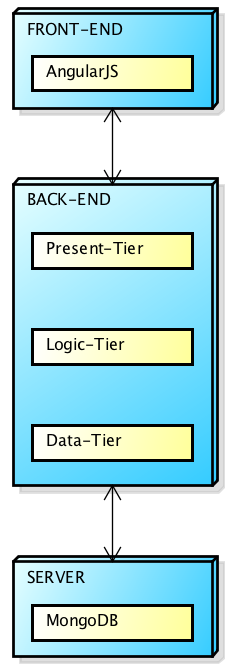
\includegraphics[width=0.2\linewidth]{img/architettura_generale_three}
		\caption[Three Tier - Premi]{Three Tier - Premi}
	\end{figure}
\end{itemize}